\documentclass[a5paper,11pt]{article}


%for coloring cell in a table
\usepackage[table]{xcolor}% http://ctan.org/pkg/xcolor

\usepackage{amsmath}
\usepackage{amssymb}

% for proofs  environment
\usepackage{amsthm}

% for 3d plots
\usepackage{pgfplots}
\usepackage{pgfplotstable}
\usepgfplotslibrary{patchplots}

\usepackage[backend=bibtex]{biblatex}
\bibliography{prob-set-4}

% for probability trees
\usepackage{tikz}
\usetikzlibrary{trees}

% for Venn diagrams
\usetikzlibrary{shapes,backgrounds}

% for plots
\usepackage{ pgfplots}
% inserted on suggestion in warning during compilation
\pgfplotsset{compat=1.9}

%for strikethrough text
\usepackage{soul}

%for R source code listing
\usepackage{listings}

%for block quotes
\usepackage{csquotes}

\newtheorem{thm}{Theorem}
\newtheorem{lem}[thm]{Lemma}

% For not indenting the first line of paragraphs:
\setlength{\parindent}{0pt}
% define the title
\author{John Hancock}
\title{Problem Set 4}
\begin{document}
% generates the title
\maketitle
% insert the table of contents
\tableofcontents
\section{References and License}
We are answering questions in the material from MIT OpenCourseWare
course 18.05, Introduction to Probability and Statistics.

In this document we are answering questions Orloff and Bloom ask in
\cite{slides7}.

Please see the references section for detailed citation information.

The material for the course is licensed under the terms at
\url{http://ocw.mit.edu/terms}.

We use documentation in  \cite{logicNot}, \cite{proofs}, \cite{bars},
\cite{packageClash}, \cite{curlyBrace}, \cite{cases} to write the \LaTeX source code for this document.

\section{Time to failure}
The first group of problems Orloff and Bloom have for us involve some
random variables that follow an exponential distribution.

The exponential distribution they give us to work with has probability
density function (pdf):

\begin{equation}
f\left(x \right) = \lambda e^{-\lambda x}, x \geq 0.
\end{equation}



\subsection{$P\left(X \geq x \right)$}

We know how to calculate $P\left(X < x \right)$ as a definite integral
\cite{reading5b}, therefore we will find 
$P\left( X < x \right)$, and our final result will be to find
$P\left(X \geq x \right) = 1 - P\left( X < x \right)$.

In order to calculate this probability, we will do a change of variable
similar to the technique Orloff and Bloom show in section 3.4 of
\cite{reading7}.

We change the variable in the pdf $f\left(x \right)$ to $u$; therefore we
rewrite the pdf as $f\left( u \right)$:

\begin{equation}
f\left(u \right) = \lambda e^{-\lambda u}.
\end{equation}

We use this definition, the fact that $f$ is defined for $x \geq 0$, and the 
definition of probability of continuous random variables \cite{reading5b} to 
write this equation:

\begin{equation}
P\left(X < x \right) = \int_0^x \lambda e^{-\lambda u} \,du.
\end{equation}

We substitute the integral on the right hand side of the previous equation 
with its antiderivative to get:

\begin{equation}
P\left(X < x \right) = -e^{-\lambda u} \bigg\rvert_{u=0}^x.
\end{equation}

We evaluate the the antiderivative at the limits of integration:

\begin{equation}
P\left(X < x \right) = -e^{-\lambda x} - -e^{-\lambda 0}.
\end{equation}

Now we simplify the previous equation:

\begin{equation}
P\left(X < x \right) = -e^{-\lambda x} + 1.
\end{equation}

Now, we apply the identity:

\begin{equation}
P\left(X \geq x \right) = 1 - P\left(X < \right).
\end{equation}

Therefore
\begin{equation}
P\left(X \geq x \right) = 1 - \left( -e^{-\lambda x} + 1 \right).
\end{equation}

The previous equation simplifies to:

\begin{equation}
P\left(X \geq x \right) = e^{-\lambda x}.
\end{equation}

\subsection{CDF of Minimum of two exponential random variables}

In this section Orloff and Bloom ask us to find the cumulative distribution
function (CDF) of two independent random variables $X_1$, and $X_2$ that both
follow an exponential distribution, and that both have mean 
$\frac{1}{\lambda}$.

In \cite{reading5c} Orloff and Bloom state that the mean of a random
variable that has probability mass function (pmf) $\lambda e^{-\lambda x}$
is $\frac{1}{\lambda}$.

Therefore $X_1$, and $X_2$ both have pmf's $\lambda e^{-\lambda x}$.

For this problem, Orloff and Bloom let $T=\text{min}\left(X_1, X_2 \right)$.

They ask us for the cdf of $T$.

The cdf of $T$ is a function $F\left(t \right) = P \left(T < t \right)$.

In the previous section, we found that for a random varialbe $X$ that has pdf
$\lambda e^{-\lambda x}$, 

\begin{equation}
P\left(X \geq x \right) = e^{-\lambda x}.
\end{equation}

We use the definition of $T$ to write the equation:

\begin{equation}
P\left(T \geq t \right) = 
  P \left(\text{min}\left(X_1, X_2\right) \geq t\right).
\end{equation}


$T=\text{min}\left(X_1, X_2 \right)$, so $T \geq t$ if, and only if, 
$X_1 \geq t$, and $X_2 \geq t$.

\begin{lem}
If two events $A$ and $B$ have a biconditional relation, then

\begin{equation}
P\left(A \right) = P \left( B \right).
\end{equation}

\begin{proof}
The proof is by contradiction.  Assume events $A$ and $B$ are biconditionally
related, but $P\left(A \right) \neq P\left( B \right)$.  Then there would
be unequal chances of events $A$ and $B$ occuring, which means that one event
would occur while the other does not.  But $A$ and $B$ are biconditionally
related, so event $A$ occurs when, and only when, event $B$ occurs. This 
is a contradiction, so $P\left(A \right) = P\left( B \right)$.
\end{proof}
\end{lem}

Therefore
\begin{equation}
P\left(T \geq t \right) = 
  P \left(X_1 \geq t, X_2 \geq t \right).
\end{equation}

$X_1$ and $X_2$ are independent events.  In \cite{reading7} Orloff and Bloom
state that random variables $X_1$ and $Y_1$ are independent if and only if:
\begin{equation}
P\left(X_1, X_2 \right)=F_{X_1}\left(x_1 \right)F_{X_2}\left(x_2\right).
\end{equation}

$F \left(X_1, X_2\right)$ is the cdf of $X_1$, and $X_2$.  
$F_{X_1}\left(x_1 \right)$, and $F_{X_2}\left( x_2 \right)$ are the marginal 
cumulative distribution functions of $X_1$, and $X_2$. 

We know that $X_1$, and $Y_1$ are exponentially distributed random variables 
with mean $\frac{1}{\lambda}$.  The answer we find in the previous section 
implies that the cdf of $X_1$ is $F_{X_1}\left(x_1 \right) = e^{-\lambda x_1}$, and the cdf of $X_2$ 
is $F_{X_2}\left(x_2 \right) = e^{-\lambda x_2}$.

Since $X_1$, and $X_2$ are independent, 

\begin{equation}
F\left(X_1, X_2 \right)= e^{-\lambda x_1} e^{-\lambda x_2}.
\end{equation}

We add the exponents of the base $e$ to simplify the previous equation to:

\begin{equation}
F\left(X_1, X_2 \right)= e^{-\lambda \left(x_1 + x_2\right)}.
\end{equation}

We are finding the cdf of $T$.

Consider $F\left(X_1 < t, X_2 < t \right)$.  We use the previous equation
to write:

\begin{equation}
F\left(X_1 < t, X_2 < t \right)= e^{-\lambda 2t}.
\end{equation}

Since $P\left(T < t \right) = P\left(X_1 < t, X_2 < t \right)$:

\begin{equation}
F\left(T < t, X_2 < t \right)= e^{-\lambda 2t}.
\end{equation}

\subsection{Three lightbulbs}

In this section we answer a question about three lightbulbs, $B1$, $B2$, and
$B3$, where each lighbulb's lifetime is an exponential random variable with
mean values $\frac{1}{2}$, $\frac{1}{3}$, and $\frac{1}{5}$, respectively.
The unit for each mean value is years.

Furthermore, Orloff and Bloom state that the lifetimes of the lightbulbs are
independent.


Let $X_1$, $X_2$, and $X_3$ be the random variables equal to the lifetimes
of $B_1$, $B_2$, and $B_3$, respectively.

Since the mean value of $X_1$ is $\frac{1}{2}$, and $X_1$
follows an exponential distribution,  $X_1 \sim 2e^{-2t}$.

Similarly, $X_2 \sim 3e^{-3t}$, and $X_3 \sim 5e^{-5t}$


We apply logic similar to what we use in the previous question to state
that the cdf of a random variable $T=\text{min}\left(X_1, X_2, X_3 \right)$
is 

\begin{equation}
F\left(T < t \right) = 
	e^{-1 \left(2+ 3 + 5\right) t }
   = e^{-10t}.
\end{equation}

The expected value of a random variable with cdf $e^{10t}$
is $\frac{1}{10}$ year.

\section{Aching Joints}

We deal with the joint distribution of two
continuous random variables $X$, and $Y$.
The probability density function for X, 
and Y is $f\left(x \right) = 
c\left(x^2+xy \right)$. 
Furthermore, $f$ is defined on 
$\left[0,1 \right] \times 
\left[0,1 \right]$.

\subsection{Value of c}
The first thing Orloff and Bloom ask us for
is the value of $c$ in $f$ as defined
above.

In order for $f \left(x, y \right)$ to be a
probabilty distribution function (PDF),
\begin{equation}
c \int_0^1 \int_0^1 x^2 + xy \,dx \,dy
= 1.
\end{equation} 

This is true, if and only if:

\begin{equation}
c \int_0^1 \frac{x^3}{3} + \frac{x^2y}{2} 
\,dy \bigg\rvert_{x=0}^1
= 1.
\end{equation} 

We evaluate the anti-derivative over the
interval indicated in the equation above
to obtain:
 
\begin{equation}
c \int_0^1 \frac{1}{3} + \frac{y}{2} 
\,dy 
= 1.
\end{equation} 

We now replace the integral of the function
of $y$ above with its anti-derivative:

\begin{equation}
c \frac{y}{3} + \frac{y^2}{4} 
\bigg\rvert_{y=0}^1
= 1.
\end{equation} 

And, we now evaluate the anti-derivative
over the interval indicated in the 
equation above:

\begin{equation}
c \frac{1}{3} + \frac{1}{4} 
= 1.
\end{equation} 

Now, we simplify the previos equation:

\begin{equation}
c \frac{7}{12} = 1.
\end{equation} 

And, we solve for $c$:

\begin{equation}
c = \frac{12}{7}.
\end{equation} 

\subsection{Marginal cumulative 
distribution, and probability density 
functions}

Orloff and Bloom are asking us to find four 
functions
\begin{itemize}
\item the marginal CDF $F_{Y} \left( y
  \right)$,
\item the marginal CDF $F_{X} \left( x
  \right)$.
\item the marginal PDF $f_{Y} \left( y
  \right)$, and
\item the marginal PDF $f_{X} \left( x
  \right)$.
\end{itemize}

The definition of marginal CDF dictates
that we evaluate the CDF at the upper 
limit of the variable that we are not
finding the marginal CDF for.

Therefore, 
\begin{equation}
F_{Y} \left(y \right) = F \left(1,y \right).
\end{equation}

In order to find the marginal CDF's, we
need to find the anti-derivative of the
PDF:

\begin{equation}
F\left( x, y \right) =
\int \int \frac{12}{7} xy + x^2 \,dx \,dy.
\end{equation}

First we find the anti-derivative with
respect to $x$:

\begin{equation}
F\left( x, y \right) =
\int \frac{12}{7} frac{x^2y}{2}
 + frac{x^2}{2} \,dy.
\end{equation}

Next, we find the anti-derivative with
respect to $y$:

\begin{equation}
F\left( x, y \right) =
\frac{12}{7} \frac{x^2y^2}{2}
 + \frac{x^2y}{2}. 
\end{equation}

Now that we have the CDF, we can partially
evaluate it to obtain the marginal CDF's.

\begin{equation}
F_{Y} \left(y \right) = F \left(1,y \right).
\end{equation}

We replace the right hand side of the 
equation above with the CDF we found, and
replace $x$ with the value 1 to find
the CDF for $y$.

\begin{equation}
F_{Y} \left(y \right) = 
\frac{12}{7} \frac{y^2}{2}
 + \frac{2y}{2}. 
\end{equation}

\begin{equation}
F_{X} \left(x \right) = F \left(x,1 \right).
\end{equation}

We replace the right hand side of the 
equation above with the CDF we found, and
replace $y$ with the value 1 to find
the CDF for $X$.

\begin{equation}
F_{Y} \left(y \right) =
 \frac{12}{7} \left(\frac{x^2}{2}
 + \frac{x^2}{2} \right). 
\end{equation}

The expression above simplifies to:

\begin{equation}
F_{Y} \left(y \right) =
 \frac{12 x^2}{7}. 
\end{equation}

Now we move on to deriving the marginal
PDF's.  We use the definition of 
marginal PDF from \cite{reading7}.

First we tackle the marginal PDF 
$f_X \left( x \right)$. 
\begin{equation}
f_{X}\left(x \right) =
\int_{0}^1 \frac{12}{7} 
  \left(x^2 + xy + \right) \,dy
\end{equation}

We replace the function with its 
anti-derivative:

\begin{equation}
f_{X}\left(x \right) =
\frac{12}{7} 
  \left(x^2y + \frac{xy^2}{2} + \right) 
  \bigg\rvert_{y=0}^1. 
\end{equation}

Now we evaluate the anti-derivative for the
interval $\left[0, 1 \right]$.

\begin{equation}
f_{X}\left(x \right) =
\frac{12}{7} 
  \left(x^2 + \frac{x^2}{2} + \right). 
\end{equation}

This is the marginal PMF 
$f_{X}\left( x \right)$.

We do a similar integration to derive the
marginal PDF $f_{Y}\left(y \right)$.

\begin{equation}
f_{Y}\left(y \right) =
\frac{12}{7} 
  \left( \int_0^1 x^2 + xy \,dx \right).
\end{equation}

We replace the integral in the equation
above with its anti-derivative.

\begin{equation}
f_{Y}\left(y \right) =
\frac{12}{7} 
  \left( \frac{x^3}{3} + frac{x^2y}{2}
 \bigg\rvert_{0}^{1}\right).
\end{equation}


We evaluate the anti-derivative over the
interval $\left[0, 1\right]$.

\begin{equation}
f_{Y}\left(y \right) =
\frac{12}{7} 
  \left( \frac{1}{3} + frac{y}{2} \right).
\end{equation}

This is the marginal PDF for 
$f_Y\left(y \right)$.

\subsection{$E\left(X \right)$, and 
Var$\left(X \right)$}

In order to calculate $E\left(X \right)$,
we integrate the product of the 
PDF $f\left(x, y \right)$, and $x$.

\begin{equation}
E\left( X \right) =
int_0^1 int_0^1 x \frac{12}{7} \left(  
x + xy
\right)\,dx.
\end{equation}

We distribute $x$ in the expression above.

\begin{equation}
E\left( X \right) =
int_0^1 int_0^1  \frac{12}{7} 
  \left(x^2 + x^2y + \right)\,dx \,dy. 
\end{equation}

First, we integrate with respect to
$x$.

\begin{equation}
E\left( X \right) =
int_0^1  \frac{12}{7} 
  \left(\frac{x^3}{3} + \frac{x^3y}{3} 
 \bigg\rvert_{x=0}^1 \right)\,dy. 
\end{equation}

Next we integrate with respect to $y$:

\begin{equation}
E\left( X \right) =
 \frac{12}{7} 
  \left(\frac{x^3y}{3} + \frac{x^3y^2}{6} 
  \bigg\rvert_{x=0}^1 
  \bigg\rvert_{y=0}^1 
 \right). 
\end{equation}

We evaluate the expression at the limits
of integtation specified to compute:

\begin{equation}
E \left(X \right) =
\frac{12}{7} \left(
  \frac{1}{3} + \frac{1}{6} \right)
  = \frac{6}{7}.
\end{equation}

In order to compute the variance of $X$,
we use the identity
\begin{equation}
\text{Var} \left(X \right) =
E \left(X^2 \right) + E \left(X \right)^2
\end{equation}

We integrate the product of $X^2$, and
the PDF Orloff and Bloom give us in
order to calculate $E \left(X^2 \right)$.

\begin{equation}
E \left(X^2 \right)  =
\int_0^1 \int_0^1 x^2 \frac{12}{7} \left(
x+xy \right) \,dx \,dy. 
\end{equation}

We distribute the $x^2$ term in the
expression above to aid in determining
the anti-derivative of the integrals.

\begin{equation}
E \left(X^2 \right)  =
\int_0^1 \int_0^1  \frac{12}{7} \left(
x^3 + x^2y \right) \,dx \,dy. 
\end{equation}

First we replace the inner integral with its
anti-derivative with respect to $x$:

\begin{equation}
E \left(X^2 \right)  =
\int_0^1 \frac{12}{7} \left(
\frac{x^4}{4} + \frac{x^3y}{3} 
\right) \bigg\rvert_{x=0}^1\,dy. 
\end{equation}

Next, we replace the remaining integral
with its anti-derivative:

\begin{equation}
E \left(X^2 \right)  =
 \frac{12}{7} \left(
\frac{x^4y}{4} + \frac{x^3y^2}{6} 
\right) \bigg\rvert_{x=0}^1 
\bigg\rvert_{x=0}^1.
\end{equation}

Now we evalute the anti-derivatives to
complete the integration:

\begin{equation}
E \left(X^2 \right)  =
\frac{12}{7}\left(\frac{1}{4}
+ \frac{1}{6} \right).
\end{equation}

We simplify the expression above to:

\begin{equation}
E \left(X^2 \right)  =
\frac{5}{7}.
\end{equation}

Now that we know $E\left(X^2 \right)$,
we can calculate Var$\left(X \right)$.

\begin{equation}
\text{Var}\left(X \right)=
E\left(X^2 \right) -
E \left(X \right)^2.
\end{equation}

We substitute the values for 
$E\left(X^2 \right)$, and 
$E\left(X \right)^2$ in the equation above
to obtain:

\begin{equation}
\text{Var}\left(X \right)=
\frac{5}{7} -
\left( \frac{6}{7} \right)^2
\end{equation}

\subsection{Variance and Covariance of
$X$ and $Y$}

In order to compute the variance and 
covariance of $X$, and $Y$, we will use
the property of covariance:

\begin{equation}
\text{Cov} = E \left(XY \right) 
- \mu_x\mu_y
\end{equation}

However, in order to use the property, 
we must calculate $\mu_y$, and 
$E\left(XY \right)$. Note that we computed
$mu_x$, in the previous section.

We use the definition of expected value
from \cite{reading6a} to compute $mu_y$.

\begin{equation}
\mu_y = int_0^1 int_0^1 y \frac{12}{7} 
\left(
x^2 + xy \,dx \,dy  \right). 
\end{equation}


We distribute $y$ in order to determine
what the anti-derivative is for the
intrgral above:

\begin{equation}
\mu_y = int_0^1 int_0^1  \frac{12}{7} 
\left(
x^2y + xy^2 \,dx \,dy  \right). 
\end{equation}

We replace the integrals above with their
anti-derivatives:

\begin{equation}
\mu_y = \frac{12}{7} 
\left(
\frac{x^3y^2}{6} + \frac{x^2y^3}{6} 
\bigg\rvert_{x=0}^1 \bigg\rvert_{x=0}^1
 \right). 
\end{equation}

And we evaluate the anti-derivative at the
limits above to obtain:

\begin{equation}
\mu_y = \frac{12}{7} 
\left(
\frac{1}{6} + \frac{1}{6} 
 \right). 
\end{equation}

The equation above simplifies to:

\begin{equation}
/mu_y = \frac{4}{42}. 
\end{equation}

We continue to collect components of the
sum we will compute in order to calculate
Cov$\left(X,Y \right)$.

We resort to the definition of expected
value in order to compute 
$E\left( X,Y \right)$

\begin{equation}
E\left( X,Y \right)=
\int_0^1 \int_0^1
\frac{12}{7} xy \left(x^2 + xy \,dx \,dy
\right).
\end{equation}

We distribute $xy$ in order to find
the anti-derivatives of the integrals
above:

\begin{equation}
E\left( X,Y \right)=
\int_0^1 \int_0^1
\frac{12}{7} \left(x^3y + x^2y^2 \,dx \,dy
\right).
\end{equation}

Now we replace the integrals above with 
their anti-derivatives:

\begin{equation}
E\left( X,Y \right)=
\frac{12}{7} \left(
\frac{x^4y^2}{8} + \frac{x^3y^3}{9}
\bigg\rvert_{x=0}^1 \bigg\rvert_{y=0}^1
\right).
\end{equation}

We now evaluate the expression above at
the limits of integration to find:

\begin{equation}
E\left( X,Y \right)=
\frac{12}{7} \left(
\frac{1}{8} 
+ \frac{1}{9} 
\right).
\end{equation}

This equation above simplifies to:

\begin{equation}
E\left( X,Y \right)=
\frac{17}{42}
\end{equation}

We now have all the components we need to
compute Cov$\left(X,Y \right)$.

\begin{equation}
\text{Cov} = E \left(XY \right) 
- \mu_x\mu_y
\end{equation}

We substitute the values we computed
previously into the equation above:

\begin{equation}
\text{Cov} =  \frac{2}{63} -
\frac{5}{7} \frac{5}{7}
\end{equation}

The above simplifies to:

\begin{equation}
\text{Cov} =  \frac{211}{567}
\end{equation}

\section{Elections}
In this section we deal with an election
scenario, and a poll of 400 people. In the
population: 0.5 of the people support
Erika, 0.2 support Ruthi, and the
remaining 0.3 support Peter, John or
Jerry.

\subsection{Apply Central Limit Theorem}
Orloff and Bloom ask us for the probabilty
that if we poll 400 people, at least 
$\%52.5$ prefer Erika. Furthermore, they 
ask us to use the central limit theorem 
to estimate the probabilty.

We treat the response of the $i^th$ person
polled $X_i$ as a Bernoulli$\left(0.5\right)$
random variable. 

We are looking for the probability that
the sum:
\begin{equation}
\sum_{i=1}^{n} x_i = (0.525)400 = 210. 
\end{equation}

We will refer to this sum as $S$. Then:
\begin{equation} \label{probS}
P \left(S > 210 \right) = 
P \left( \frac{S - \mu}{\sigma} > 
\frac{210- \mu}{\sigma}\right).
\end{equation}

Note: if $S$ has mean $\mu$, then 
$S-\mu$ has mean 0. We cite properties of
expexted value in \cite{reading4b} for
the explanation that $S-\mu$ has mean 0.

Also note: if  $S$ has standard deviation
$\sigma$ then $\frac{S}{\sigma}$ has 
standard deviation 1. We use the
property of variance \cite{reading5b}:
\begin{equation}
\text{Var}\left( aX  + b \right) =
a^2 \text{Var}\left(X \right).
\end{equation}
Here we let $a=\frac{1}{\sigma}$.
Then
\begin{equation}
\text{Var}\left(\frac{S}{\sigma}
\right) =
\frac{1}{\sigma^2}
\text{Var}\left( S \right).
\end{equation}

We beg the reader to bear in mind that
the standard deviation of $S$ is 
$\sigma$.

By definition, variance is the square
of standard deviation, so the
expressions on both sides of the equation
above are equal to $1$.

In order to procede, we must compute the
mean, and standard deviation of $S$.

We define $S$ as the sum of 400
Bernoulli$\left(0.5 \right)$ random
variables, $X_i$.  We know from 
\cite{reading4b} that the expected
value of $X_i$ is $0.5$. \cite{reading4b}
also tells us that the expected value
of the sum of the $X_i$ is 200. 


In \cite{reading5a},
Orloff and Bloom show the variance of
a random variable 
$X \sim \text{Binomial}\left(n, p \right)$
is $np\left(1-p\right)$.

Therefore the variance of $S$ is 
\begin{equation}
400\times0.5\times0.5=100.
\end{equation}

Since standard deviation is the square root
of variance, the standard deviation
$\sigma_S$ of $S$ is $10$.

Now that we have computed the mean and
standard deviation of $S$, we can 
substitute them into \ref{probS}: 

\begin{equation} 
P \left(S > 210 \right) = 
P \left( \frac{S - 200}{10} > 
\frac{210- 200}{10}\right).
\end{equation}

The equation above simplifies to:

\begin{equation} 
P \left(S > 210 \right) = 
P \left( \frac{S - 200}{10} > 
1 \right).
\end{equation}

We may apply the central limit theorem 
to write:

\begin{equation} 
P \left( \frac{S - 200}{10} > 1
\right) \approx
P \left(Z > 1 \right).
\end{equation}

We use the rule of rule of thumb 
\cite{reading6b}and the expression
above to ascertain

\begin{equation} 
P \left( \frac{S - 200}{10} > 1
\right) \approx
0.68
\end{equation}

Recalling \ref{probS} we see it is the case
that:

\begin{equation} \label{probS}
P \left(S > 210 \right) \approx 
0.68.
\end{equation}

\subsection{Apply central limit theorem again}
Now, we turn our attention to the question
of what would be the probabilty that at
least $0.25$ of 400 people polled support
Peter, Jon, or Jerry.

We define a new sum of random variables

\begin{equation}
S = \sum_{n=1}^{400} X_i 
\end{equation}

Where each of the $X_i$ is a Bernoulli
random variable that takes the value of
1 with a probabilty of $\frac{1}{3}$,
and 0 otherwise.

We define the $X_i$ in this way because
$0.3$ of the population support Peter,
Jon, or Jerry. 

Moreover \cite{reading5a} explains that
the mean (expected) value of $S$ is 
$\mu_S = 400 \times 0.3 = 120$, and that
the variance of $S$ is
$400 \times 0.3 \times 0.7 = 84$.
Hence the standard deviation $\sigma_S$ of 
$S$ is $sqrt{84} \approx 9.165$.


In this case we are looking for

\begin{equation}
P\left(S < 100\right)
\end{equation}

We use the same reasoning as in the
previous section to conclude:

\begin{equation}
P\left(S < 100\right) =
P\left(\frac{S-120}{9.165} < 
\frac{100-120}{9.165} \right).
\end{equation}

And we are in a position to use the central
limit theorem to obtain:

\begin{equation}
P\left(\frac{S-120}{9.165} < 
\frac{100-120}{9.165} \right) \approx
P\left(Z < -2.182 \right)
\end{equation}

The rule of thumb \cite{reading6b} tells us
that there is a 95\% probabilty that $Z$
will be within two standard deviations of
the mean. Since $Z$ has standard deviation
1, there is a 5\% chance $Z$ will have a
value larger than $2$, or smaller than 2.
The normal distribution is symmetric
with respect to the $x$ axis, so the chance
$Z$ is less than $2$ is 0.025.

We can get a more precise answer using R.
In R, qnorm$\left( -2.182 \right) = 
0.01455477$.

\section{Rounding Error}
In this section we address the problem
Orloff and Bloom pose regarding rounding
error, where we round 1,000 random amounts
of money to the nearest nickel.

We model the rounding error as a random
variable $X_i, i \in 1, 2, \ldots, 1,000$ from a uniform distribution
from the set of values: 
$\left\{-2,-1,0,1,2 \right\}$.


We define $S$ to be the sum of the $X_i$.
In order to apply the central limit theorem
we must find the mean $\mu_S$, and standard
deviation $\sigma_S$ of $S$.

Each of the $X_i$ is uniformly distributed from a set 
of 5 values; therefore the expected value
of $X_i$ is:
\begin{equation}
0.2\left(-2 \right) +
0.2\left( -1 \right) +
0.2\left( 0  \right) +
0.2\left( 1 \right) +
0.2\left( 2 \right) =
0
\end{equation}

Therefore the expected value of $S$ is also 0.

We use the formula for variance of a
uniformly distributed random variable 
from \cite{reading5a}. 

In this case, 
\begin{equation}
Var\left(X_i \right) =
\frac{24}{12} = 2. 
\end{equation}

Since $S$ is the sum of the $X_i$, Var$\left(S \right)=2,000$.

Hence, $\sigma_S = \sqrt{2,000}$.

Orloff and Bloom ask us to use the central limit theorem to estimate
\begin{equation}
P\left(S > 100 \right).
\end{equation}

We standardize the event above to an event of equal probabilty:
\begin{equation}
P\left(S > 100 \right)=
P\left(\frac{S-\mu_S}{\sigma_S} > 
\frac{100 - \mu_S}{\sigma_S} \right).
\end{equation}

We determined $\mu_S$ and $\sigma_S$, so
we substitute those values in the
expression above to get:

\begin{equation}
P\left(S > 100 \right)=
P\left(\frac{S}{\sqrt{2000}} > 
\frac{100}{\sqrt{2000}} \right).
\end{equation}

We simplify the right hand side of the
inequality above to:

\begin{equation}
P\left(S > 100 \right)=
P\left(\frac{S}{\sqrt{2000}} > 
2.236 \right).
\end{equation}

We are now in a position to apply the
central limit theorem \cite{reading6b}. 
$S$ is the sum of
independent identically distributed
random variables, and we normalize $S$ in 
such a way that it has mean $0$ and
standard deviation $1$. Hence, we apply
the central limit theorem, and approximate:

\begin{equation}
P\left(S > 100 \right) \approx
P \left(Z > 2.236 \right).
\end{equation}

Where $Z$ follows the normal distribution
$N\left(0,1 \right)$.

We use the pnorm function of the R 
programming language to find 
$P \left(Z > 2.236 \right) 
\approx .0254$.

The R code we write to obtain the 
probabilty above is:
\begin{lstlisting}
(1- pnorm(2.236))*2
\end{lstlisting}

To summarize, there is approximately
a 0.025 probability that the rounding
error will be greater than or equal to
100 cents.

\section{Independence}
Orloff and Bloom give us a joint distribution of two random  variables
$X$, and $Y$, and ask us to determine whether or not they are independent.

In \cite{reading7} Orloff and Bloom state 
that two random variables in a joint
distribution are independent if the
probability of every possible combination
of the random variables is the product
of the respective marginal probabilities of
the combination.

Therefore we will extend the table Orloff
and Bloom give for this problem to
include the marginal probabilities:


\begin{center}
\begin{tabular}{ | c | c | c | c  | c | }
    \hline
    $X$/$Y$ & 1 & 2 & 3 & $f_X$ \\ \hline
    1 & $\frac{1}{18}$ & $\frac{1}{9}$ & $\frac{1}{6}$ & $\frac{1}{3}$ \\ \hline
    2 & $\frac{1}{9}$ & $\frac{1}{6}$ & $\frac{1}{18}$ & $\frac{1}{3}$ \\ \hline
    3 & $\frac{1}{6}$ & $\frac{1}{18}$ & $\frac{1}{9}$ & $\frac{1}{3}$ \\ \hline
    $f_Y$ & $\frac{1}{3}$ & $\frac{1}{3}$ & $\frac{1}{3}$ & 1 \\ \hline
  \end{tabular}
\end{center}

We see in the table above that the marginal probabilities are all $\frac{1}{3}$.
Therefore, the product of any pair of marginal probabilities is $\frac{1}{9}$.
However, there are entries in the table
above that are not $\frac{1}{9}$. Therefore
$X$, and $Y$ are not independent.

\section{Correlation}
Orloff and Bloom give the following
distribution for this problem:

\begin{center}
\begin{tabular}{ | c | c | c | c  |  }
    \hline
    $X$/$Y$ & -1 & 1 & $f_X$ \\ \hline
    -1 & $c$ & $\frac{1}{2} -c$ & $\frac{1}{2}$ \\ \hline
    1 & $\frac{1}{2} -c$ & $c$ & $\frac{1}{2}$ \\ \hline
    $f_Y$ & $\frac{1}{2}$ & $\frac{1}{2}$ & 1 \\ \hline
  \end{tabular}
\end{center}

\subsection{Compute Covariance}
We use the property of covariance from \cite{reading7b}:
\begin{equation}
\text{Cov}\left(XY\right) = E\left(XY \right)-\mu_X\mu_Y.
\end{equation}

Evidently, it is necessary to derive 
$E\left(XY \right)$, $E\left(X\right)$,
and $E\left(Y\right)$, in order to 
determine the covariance of $X$, and $Y$.

\begin{equation}
E\left(XY\right)=
\sum_{i=1}^2 \sum_{j=1}^2 x_i y_j 
p \left(x_i, y_j \right).
\end{equation}

We use the distribution in the table
above to compute this expexted value.

\begin{equation}
E\left(XY\right)=
\left(-1\right)\left(-1\right)c +
\left(-1\right)\left(1\right)\left(\frac{1}{2} -c\right) +
\left(-1\right)\left(1\right)\left(\frac{1}{2} -c\right) +
\left(1\right)\left(1\right)c.
\end{equation}

We can simplify the right hand side to:

\begin{equation}
E\left(XY\right)=
4c - 1.
\end{equation}

We need the expected value of $X$, and
$Y$ as well. The expected value $\mu_X$
of $X$ is:

\begin{equation}
E\left(X\right) =
\sum_{i=1}^{2} \sum_{j=1}^2 
x_i p\left(x_i, y_j \right).
\end{equation} 

This sum is:

\begin{equation}
E\left(X\right) =
\left(-1\right) c +
\left(1\right) \frac{1}{2} - c+
\left(-1\right) \frac{1}{2} - c+
\left(1\right) c. 
\end{equation} 

The right hand side of the equation above
simplifies as follows:

\begin{equation}
E\left(X\right) =
0.
\end{equation}

The the values for $Y$ in this problem are
such that we calculate $\mu_Y$ to have
the same value as we find for $\mu_X$. 
Hence, $E\left(Y\right)=0$.

Therefore Cov$\left(X,Y\right)=4c-1$.

\subsection{Calculate Correlation}
In order to calculate the correlation of
$X$, and $Y$, we must find the standard
deviation of $X$, and $Y$.

We use the property of variance from
\cite{reading5a}:

\begin{equation}
\text{Var}\left(X\right) =
E\left(X^2\right) -
E\left(X\right).
\end{equation}

We know from our calculations in the 
previous section that $E\left(X\right)$,
and $E\left(Y\right)$ are both equal to
$0$.

Therefore we only need to calculate 
$E\left(X^2\right)$, and 
$E\left(Y^2\right)$.

\begin{equation}
E\left(X^2\right) =
\sum_{i=1}^{2} \sum_{j=1}^2 
x_i^2 p\left(x_i, y_j \right).
\end{equation} 

This sum is:

\begin{equation}
E\left(X\right) =
\left(-1\right)^2 c +
\left(1\right)^2 \frac{1}{2} - c+
\left(-1\right)^2 \frac{1}{2} - c+
\left(1\right)^2 c. 
\end{equation} 

The right hans side of the equation above
simplifies to:

\begin{equation}
E\left(X\right) = 1.
\end{equation} 

Similar calculations would show that
$E\left(Y\right)=1$.

Therefore Cor$\left(X,Y\right) = 4c-1$.

\subsection{Independence, correlation}

In this section we answet the questions
Orloff and Bloom ask about which values
of $c$ in the distributon they give
us for the problem make $X$, and
$Y$ independent, and which values
make $X$, and $Y$ 100\% correlated.

In order for $X$, and $Y$ to be 
independent, each probability in the
table above must be the product of the 
marginal probabilities for the row
and column that the probability is in.

All of the marginal probabilities are
$\frac{1}{2}$, so in order for $X$, and
$Y$ to be independent $c$  and $\frac{1}{2}
-c$ must both equal $\frac{1}{4}$. If $c$
equals $\frac{1}{4}$, then $\frac{1}{2} - c
= \frac{1}{4}$. Hence $X$, and $Y$ are 
independent when $c=\frac{1}{4}$.

In order for $X$, and $Y$ to be 100\%
correlated, Cor$\left(X,Y\right) = 1$.
Above, we determine: 

\begin{equation}
\text{Cor}\left(X,Y\right) = 4c -1
\end{equation}

Therefore, $X$, and $Y$ are 100\% 
correlated when $c=\frac{1}{2}$.

\section{Joint Uniform Distribution}

In this section, we are dealing
with joint, independent, uniformly
distributed random variables A and B. 

A and B are both uniformly distributed on
$\left[0,60\right]$.

\subsection{Joint distribution functions}
$A$, and $B$ are independently, uniformly
distributed random variables. There is a 
one in 60 chance that $A$ takes a 
certain value, and likewise for $B$.
Therefore, the probabilty that $A$, and
$B$ take a specific pair of values is
$\frac{1}{3,600}$.

Therefore the joint pdf for $A$, and $B$
is:

\begin{equation}
f\left(a, b \right) = \frac{1}{3600}.
\end{equation}

Orloff and Bloom give us that $A$, and $B$
are defined on $\left[0,60\right]$. We 
assume this is a closed subset of the real
numbers. Therefore we treat $A$, and $B$ as
continuous random variables.

The joint cdf is:
\begin{equation}
F\left(a,b\right)=
\int_{0}^{a} \int_{0}^{b}
\frac{1}{3600} \,dx \,dy.
\end{equation}

We replace the integrals above with their
anti-derivatives:

\begin{equation}
F\left(a,b\right)=
\frac{ab}{3600} \bigg\rvert_0^a
\bigg\rvert_0^b.
\end{equation}

\subsection{Probability for A}
Orloff and Bloom ask us to calculate the
probability that $A$ is less than $1,800$.

\begin{equation}
P\left(A<30\right)=int_0^{30} \frac{1}{60}.
\end{equation}

This integral evaluates to $\frac{1}{2}$.

\subsection{Probability for $A$ and $B$}

We find the probability that 
$0 \leq A \leq 15$, and
$30\leq B \leq 45$.

$A$ and $B$ are independent, therefore 
\begin{equation}
P\left(0 \leq A \leq 15 \text{and} 
30 \leq B \leq 45 \right) =
P\left(0 \leq A \leq 15 \right) 
P\left(30 \leq B \leq 45\right).
\end{equation}

Since $A$, and $B$ are uniformly
distributed on $\left[0, 60 \right]$, 
$P\left(0 \leq A \leq 15\right)=\frac{15}{60}$, and 
$P\left( 30 \leq B \leq 45\right) = \frac{15}{60}$.

Therefore the 
\begin{equation}
P\left(0 \leq A \leq 15 \text{and} 
30 \leq B \leq 45 \right) =
\left(\frac{1}{4}\right) \left(\frac{1}{4} \right).
\end{equation}

We multiply the fractions on the right hand side of the equation above
to get:

\begin{equation}
P\left(0 \leq A \leq 15 \text{and} 
30 \leq B \leq 45 \right) =
\frac{1}{8}.
\end{equation}

\subsection{Inequality probability}
In this section, we will calculate the probability that $A \leq B + 5$.

Here is a plot of the inequality:
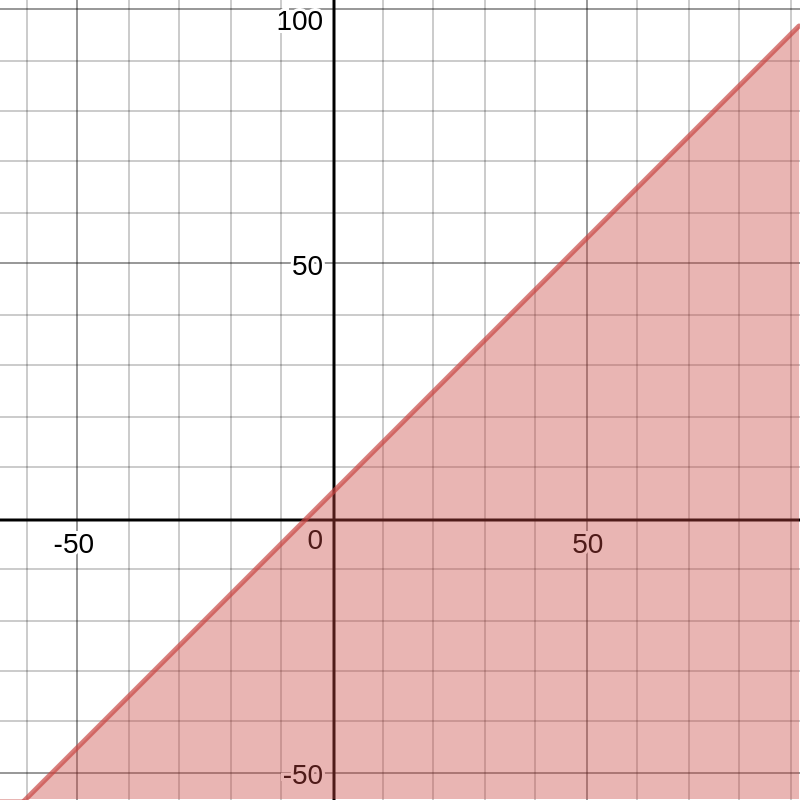
\includegraphics[scale=0.5]{alice_5_after_bob.png}

We are only interested in the region of the plane composed of points in
$\left[0,60 \right] \times \left[0,60\right]$.

Therefore we find the area of this region integrating the function
\begin{equation}
f\left(x) = x + 5.
\end{equation}

The area of the shaded region will be:

\begin{equation}
int_{0}^{55} x + 5 \,dx.
\end{equation}

We replace the integral above with its anti-derivative:

\begin{equation}
\frac{x^2}{2} + 5x \bigg\rvert_0^{55}.
\end{equation}

We evaluate at the limits of integration:

\begin{equation}
\frac{x^2}{2} + 5x \bigg\rvert_0^{55} = \frac{55^2}{2} + 5\left(55\right).
\end{equation}

The right hand side of the equation above simplifies to:

\begin{equation}
\frac{x^2}{2} + 5x \bigg\rvert_0^{55} = 1787.5.
\end{equation}


Within that region, we want to know what fraction the shaded portion is 
iof the region.

It will be easier to subtract the area of the unshaded portion from the
area of the region to find the area of the shaded portion, since the
unshaded portion is a triangle.

The unshaded portion is a right triangle, with one side of length 55, and the
other side also of length 55.  Therefore the region of the unshaded 
\printbibliography{}

\end{document}
